\chapter{Introduction}
\section{Preface}
    \textit{``We all have tremendous potential, and we all are blessed with gifts. Yet, the one thing that holds all of us back is some degree of self-doubt. It is not so much the lack of technical information that holds us back, but more the lack of self-confidence.``}
    \begin{flushright}
    -- Robert T. Kiyosaki, ``Rich Dad, Poor Dad``\\
    \end{flushright}
    %
    It is a quote from a brilliant book, written by Robert Kiyosaki -- an American businessman who's net worth is estimated at \$100 million, titled ``Rich Dad, Poor Dad``. Kiyosaki puts stress on how illiterate and uneducated the society is when it comes to, what he calls \textit{financial intelligence} -- skills and knowledge gained from understanding financial principles and ability to use them in everyday life.
    
    Inspired by the message from the book and the originality of functional programming, as well as its applicability in modeling financial models, this paper is an attempt to bring some issues from the world of finance and mathematics closer. Since the term \textit{Industry 4.0} is so broad and one of its components is widely understood automation -- I hope the \textit{MARS App} will equal to the task.
    
\section{Thesis assumptions}
    The main goal of this work is to create a tool in the functional programming paradigm which will be used to price selected financial instruments. To achieve this goal F\# programming language will be used as it was created mostly to support functional programming and a European option will be priced as an example of a derivative financial instrument.
    %
    The app will consist of several different technologies such as MVVM design pattern, XAML language to create View part of the project and minor C\# background to connect XAML's View with F\#'s ViewModel. Everything will be written in Visual Studio 2019 IDE.
    
    The basic assumptions within the application include:
    \begin{itemize}
        \item \textit{Geometric Brownian Motion} implementation as a model used for generating underlying asset prices.
        \item Opportunity to specialize the product by changing:
            \begin{itemize}
                \item maturity (expiration time),
                \item interest rate,
                \item stock's initial price,
                \item drift,
                \item volatility.
            \end{itemize}
        \item Implementing Black-Scholes model for option pricing.
        \item Preparation of the application's graphic design in XAML and connecting the View with logic.
    \end{itemize}
    
    \noindent
    Further chapters consecutively cover above issues.
    
\section{Scope of the thesis}
    The next sections in this chapter will bring closer the technologies used for the sake of the project: quick overview of the most common programming paradigms, introduction to \textit{F\#} and \textit{XAML} languages and \textit{MVVM} design pattern.
    %
    The following chapter is divided into 3 sections -- explanation of the \textit{Geometric Brownian Motion}, introduction to financial options and the \textit{Black-Scholes Model}.
    %
    Last chapter contains summary of the project assumptions and several \textit{future works} possibilities.
    
\section{Technologies Overview}
    This section describes the most important topics of the technological stack of the project.
    \subsection{Programming paradigms}\index{Paradigm}
        A programming paradigm is nothing more but an overall concept which describes \textit{how} the programming is done and what is the methodology behind the language that adheres to a specific type of a paradigm. Throughout the years programming languages evolved, new ones have been created, so that today there are from 150, according to TIOBE Programming Community, up to 700, listed by Wikipedia, different programming languages (more information can be found here \cite{numberOfProgrammingLanguages}). Although some sources, e.g. \cite{numberOfProgrammingLanguages_hopl_info}, state that there are almost as many as 9000 (sic) programming languages the exact number of those is not that important -- rather the variety and the sheer number of them is crucial as it indicates that they must differ from each other and it turns out these differences can somehow be grouped, what is presented below.
        
        The most basic and intuitive approach into dividing the paradigms into 2 basic groups seems to be this one:
        \begin{itemize}
            \item Imperative Programming,
            \item Declarative Programming.
        \end{itemize}
        The following sections present above paradigms.
    
    \subsubsection{Imperative Programming}\index{Imperative Programming}
        This way of programming is not by accident described as the first one -- historically languages that present this type of programming have emerged primarily. Imperative programming enables the programmer to manage processor's behavior on much more precise level. The commands show step-by-step how the computation is executed. These commands affect a program's state. This paradigm focuses on describing \textit{how} the goal should be achieved.
        
        Imperative programming can be further broken down into 3 groups:
        \begin{enumerate}\index{Procedural Programming}
            \item \textbf{Procedural Programming} -- the underlying model is based on a procedure (set of coded instructions, more in \cite{procedureDefinition}). It has the ability to use once written code again. The examples of procedural programming examples include:
                \begin{itemize}
                    \item C,
                    \item C++,
                    \item Java,
                    \item ColdFusion,
                    \item Pascal.
                \end{itemize} \index{OOP}
            \item \textbf{Object Oriented Programming} -- a program is a set of classes and objects (instances of a class) that are meant to interact with each other. The examples of languages supporting OOP include:
                \begin{itemize}
                    \item Objective-C,
                    \item C++,
                    \item Java,
                    \item Visual Basic .NET,
                    \item Python.
                \end{itemize} \index{Parallel Processing Approach}
            \item \textbf{Parallel Processing Approach} -- this style of programming is designed to divide computing the code into multiple processors in order to minimize the time required for computation. The examples of languages supporting parallel programming approach include:
                \begin{itemize}
                    \item NESL,
                    \item C,
                    \item C++.
                \end{itemize}
        \end{enumerate}
    
    \subsubsection{Declarative Programming}\index{Declarative Programming}
        On the other hand a programmer may want to focus not on \textit{how} the code should be ran on a computer but rather what \textit{what the result should look like} and the way of obtaining it is not the most important thing. One would rather give it up to the compiler to decide what is the best way of achieving the result. Declarative programming is also consisted of smaller groups, such as:
        \begin{enumerate} \index{Logic Programming}
            \item \textbf{Logic Programming} -- in logic programming the programmer has knowledge, expressed in a logical form, about facts and rules concerning a specific problem, more details here \cite{logicProgramming}. This type of programming resembles a mathematical proof. \textbf{Prolog} language is an example of this programming paradigm.
            
            \index{Database-Driven Programming}
            \item \textbf{Database-Driven Programming Approach} -- it is based on storing the data and moving it, as well as about keeping information about the relations among entities. \textbf{SQL} is one of the most popular examples of this programming group.
            
            \index{Functional Programming}
            \item \textbf{Functional Programming} -- like object in object-related programming in functional programming the most basic unit is a function. Shared state is avoided, as well as mutable data (the programmer is unable to crate a variable). The examples of functional programming paradigm:
                \begin{itemize}
                    \item F\#,
                    \item Haskell,
                    \item Common Lisp,
                    \item OCaml,
                    \item Racket.
                \end{itemize}
        \end{enumerate}
    
    \begin{figure}[H]
        \centering
        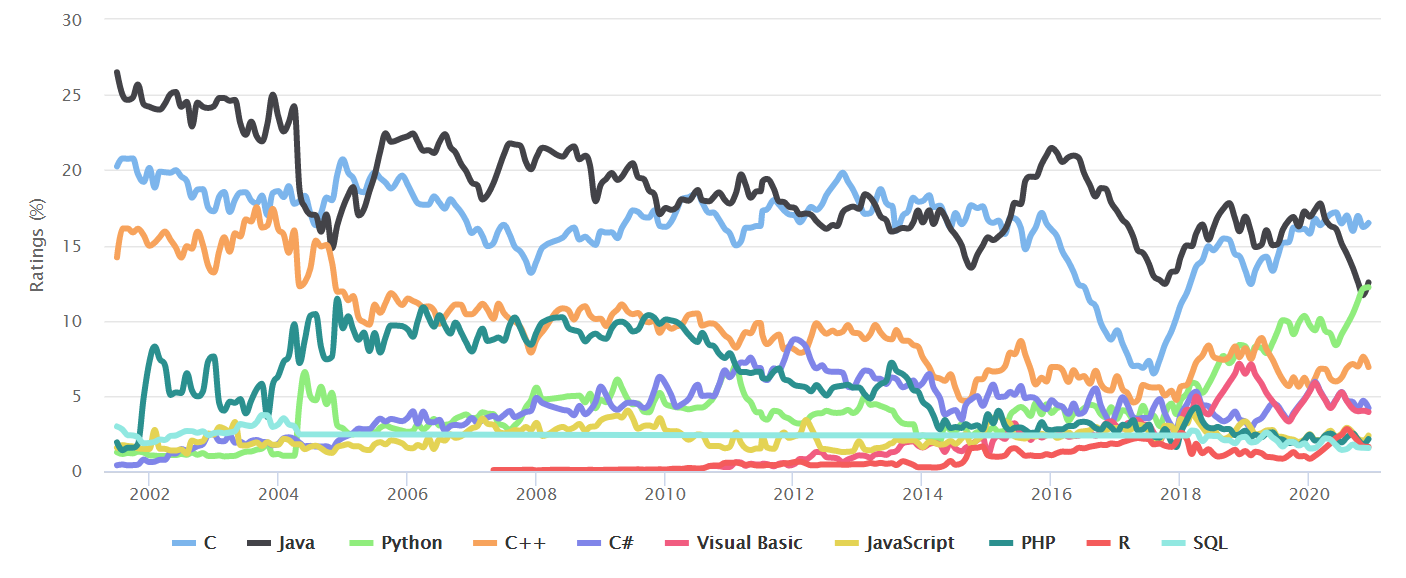
\includegraphics[width=\textwidth]{img/tiobe_index.png}
        \caption{The most popular languages and their trends.}
        \source{https://www.tiobe.com/tiobe-index/}
        % \caption*{Source: \url{https://www.tiobe.com/tiobe-index/}}
        \label{fig:tioebeIndex}
    \end{figure}
    
    \noindent
    Figure \ref{fig:tioebeIndex} presents graphical overview on popularity of the most used programming languages in recent years.

\subsection{F\# Language}\index{F\# Language}
    F\# is a programming language that was created back in 2005 by Don Syme in cooperation with Microsoft Research. Although it is a multi-paradigm programming language it best fits the functional, declarative programming group. It is open-source and belongs to .NET Framework (more information here \cite{WhatIsFSharp},  \cite{FSharpWiki}).
    
    F\# is a strongly typed language that uses type interference. It has lightweight syntax and is immutable by default. Lightweight syntax can be observed in low signal-to-noise ratio in comparison to other languages (for example C\#).
    
    \begin{lstlisting}[caption=C\# code example]
public static class SumOfSquaresHelper
{
   public static int Square(int i)
   {
      return i * i;
   }

public static int SumOfSquares(int n)
   {
      int sum = 0;
      for (int i = 1; i <= n; i++)
      {
         sum += Square(i);
      }
      return sum;
   }
}

int r = SumOfSquaresHelper.SumOfSquares(100);
    \end{lstlisting}
    
    \begin{lstlisting}[caption=F\# code example]
let sumOfSquares n = 
   [1..10] |> List.map (fun x -> x*x) |> List.sum

let r = sumOfSquares 100
    \end{lstlisting}
    
    Both above snippets are taken from the site \url{https://fsharpforfunandprofit.com/} with minor changes applied to further improve F\# code by using lambda function (snippets source \cite{compareCandF}). Both of these perform the same task -- count the sum of squares of all integers preceding a certain number. The goal is to show how succinct F\# can be in comparison to the same code but written in C\#.
    
    Taking all F\# features into account it becomes visible that it is a very interesting, high level language that has a potential to be used in various situations. One of these is mathematical modeling vastly used for financial purposes such as pricing financial instruments -- what is presented in this thesis. In order to estimate the price, a certain model has to be used and since there are so many variables nonlinearly affecting the final price -- the models are frequently quite complex. For the sake of simplifying the process of implementing the model, having a syntax that very well resembles the mathematical language is beneficial.
    
    Immutability options introduced in F\# significantly reduce the possibility of making a mistake by a programmer which could be hard to find while debugging the code. Furthermore syntax such concise as F\#'s is far more susceptible for code maintenance.
    %
    These are the major reasons why F\# was selected to be the core language of the project.
\subsection{MVVM design pattern}\index{MVVM Design Pattern}
    \textit{Model-View-ViewModel} is one of design patterns that are used in programming. It's primary role is to separate the user interface from the  back-end logic. For this purpose there are 3 main components of the MVVM pattern:
    \begin{itemize}
        \item View,
        \item ViewModel,
        \item Model.
    \end{itemize}
    
    \begin{figure}[H]
        \centering
        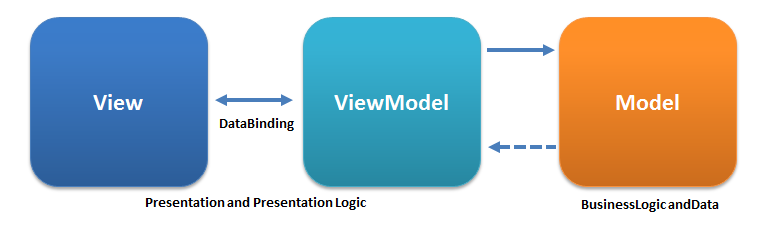
\includegraphics[width=\textwidth]{img/MVVMPattern.png}
        \caption{Three basic components of the MVVM architectural pattern.}
        \label{fig:mvvm_pattern}
        \source{https://en.wikipedia.org/wiki/Model-view-viewmodel\#/media/File:MVVMPattern.png}
    \end{figure}
    %
    The Fig. \ref{fig:mvvm_pattern} presents a graph with relations between the  components. The important point is the fact that the View ``does not see`` the Model. Components of the View are \textit{binded} with corresponding ones in the ViewModel. In the ViewModel they are specially equipped with mechanisms responsible for keeping the changes up to date (change in the logic immediately triggers change in the View part). ViewModel works as a bridge between the Model and the View.
    
    \subsubsection{View} \index{View}
        View in this case is a synonym of UI (in most cases GUI). View's purpose is to define the appearance of an app: where do buttons appear and how they look, how the data is presented to the user and which elements are static or have dynamic binding. As the name suggests, it handles the \textit{view} of an app - what can actually be seen on the screen.
        %
        In the presented application the role of the \textit{View} part is taken by a project named \textit{View} \ref{fig:view}.
        
        \begin{figure}[H]
            \centering
            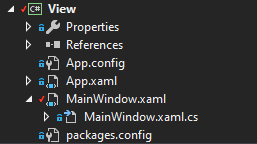
\includegraphics{img/view.png}
            \caption{\textit{View} project seen from Solution Explorer.}
            % \caption*{Source: \textit{MARS App}}
            \source{own study}
            \label{fig:view}
        \end{figure}
        
        \begin{figure}[H]
            \centering
            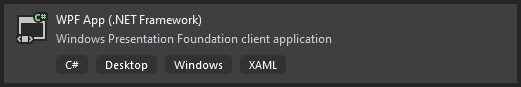
\includegraphics{img/view_wpfApp.png}
            \caption{Default Visual Studio 2019 project used for writing the \textit{View} part of an app.}
            % \caption*{Source: Microsoft Visual Studio 2019 -- Create a new project tab.}
            \source{own study}
            \label{fig:view_wpfApp}
        \end{figure}
        
        \noindent
        This project, presented in the Figure \ref{fig:view}, based on Visual Studio 2019 default project \textit{WPF App (.NET Framework)} (see Fig. \ref{fig:view_wpfApp}) is the only non-F\# part of the MARS App as, for the time being (December 2020), there is no dedicated project in the F\# language that would, by default, be compatible with MVVM architecture and XAML markup language for presenting the view. Therefore a few lines of C\# code needed to be added in order to bind successfully View project with ViewModel one.
        

    \subsubsection{Model} \index{Model}
        The \textit{Model} section handles business logic and data of the app. It is an inherent entity that could be reused in other applications. It is a significant advantage of the MVVM architectural pattern -- reusability of the code is supported at the conceptual level of the design pattern.
        
        This time \textit{Model} project, show in the Figure \ref{fig:model_VS19Project}, is solely an F\# project that targets .Net Framework 4.6.1.
        \begin{figure}[H]
            \centering
            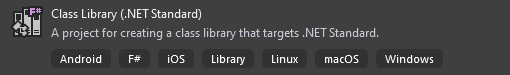
\includegraphics{img/model_VS19Project.png}
            \caption{Default Visual Studio 2019 project used for writing the \textit{Model} part of an app.}
            % \caption*{Source: Microsoft Visual Studio 2019 -- Create a new project tab.}
            \source{own study}
            \label{fig:model_VS19Project}
        \end{figure}
        
        It is useful to remind here that whenever there is no valid reason to use \textit{.NET Core} over \textit{.NET Framework}, one should always opt for the latter. \textit{.NET Core} is used when multi-platform approach is expected, but if the app is destined for Microsoft Windows system then the amount of libraries available on \textit{.NET Standard} is vastly higher.
        
        \begin{figure}[H]
            \centering
            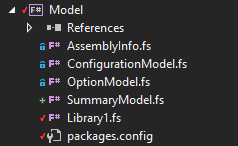
\includegraphics{img/model.png}
            \caption{\textit{Model} project seen from Solution Explorer.}
            % \caption*{Source: \textit{MARS App}}
            \source{own study}
            \label{fig:model}
        \end{figure} 
        
    \subsubsection{ViewModel} \index{ViewModel} 
        Last but surely not least the \textit{ViewModel} serves a role of a so-called \textit{bridge} between \textit{View} and the \textit{Model}. It binds the graphical presentation of the components with hidden back-end logic. It must hold a reference to the \textit{Model} project of the solution. It is extremely important for the programmer to design proper updates of data presented in corresponding graphic fields. \textit{INotifyPropertyChanged} interface is perfect for this purpose. It makes sure no change in the data filed will go unnoticed if it can be seen anywhere in the app by the user.
        
        It consists of multiple files responsible for specific purposes, all starting with the line:
        
        \begin{lstlisting}[label={lst:model1}, caption=F\# all \textit{ViewModel} project components beginning.]
namespace ViewModel
// lines of code
        \end{lstlisting}
        %
        An alternative notation would be to use F\# \textit{module} declaration, as in an example below. Such practice in more common nowadays than OOP-resembling \textit{namespace}.
        %
        \begin{lstlisting}[label={lst:model2}, caption=F\# alternative example \textit{ViewModel} project component beginning.]
module MARSApp.ViewModel.ConfigurationViewModel
open MARSApp.ViewModel.ViewModelBase
open MARSApp.Model.ConfigurationModel
// lines of code
        \end{lstlisting}
        %
        Although the difference and these code fragments \ref{lst:model1} \ref{lst:model2} may seem unimportant, there is a solid reason for choosing the first one -- since the project contains GUI written in XAML there is a need to specify in the view where certain properties can be found. It turns out there is a major problem if the properties lay hidden inside a module. When they are presented in a namespace it is easier to bind them with XAML as it is adapted to receive a \textit{namespace} declaration in the \textit{Window} heading:
        \begin{figure}[H]
            \centering
            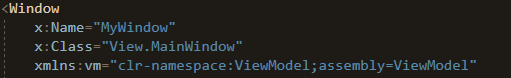
\includegraphics{img/viewmodel_namespace.png}
            \caption{Fragment of file \textit{MainWindow.xaml} showing \textit{namespace} reference.}
            % \caption*{Source: \textit{MARS App}}
            \source{own study}
            \label{fig:viewmodel_namespace}
        \end{figure}
        \begin{figure}[H]
            \centering
            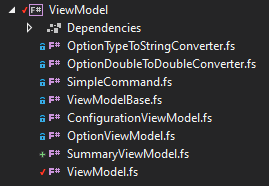
\includegraphics{img/viewmodel.png}
            \caption{\textit{ViewModel} project seen from Solution Explorer.}
            % \caption*{Source: \textit{MARS App}}
            \source{own study}
            \label{fig:viewmodel}
        \end{figure} 
        \noindent
        The reference would be much harder to achieve if \textit{module} approach was used. For the sake of implementing \textit{ViewModel} in this example the same default VS19 project was used as in \textit{Model} project.
    
\subsection{XAML Language} \index{XAML Language} \index{HTML Language} \index{JSON Format}
    \textit{XAML} stands for Extensible Application Markup Language and belongs to the declarative markup language group. It is used in \textit{WPF} (\textit{Windows Presentation Forms} -- User Interface framework for creating desktop client applications, more details here \cite{wpf}) for separating between how an application looks like and how it behaves (more how \textit{XAML} works in \cite{how_xaml_works}) (both the GUI and its behavior were created in the same language). \textit{XAML} is an subset of \textit{XML}, because every \textit{XAML} file is as well a \textit{XML} file, but not every \textit{XML} file is a \textit{XAML} file.
    
    \textit{XAML} may resemble \textit{HTML}, although the idea behind those two is utterly different -- by comparing \textit{XML} to \textit{HTML} one can observe that:
    \begin{itemize}
        \item \textit{XML} is a markup language much like \textit{HTML} but \textit{HTML} was designed to display data while \textit{XML} to carry it.
        \item \textit{HTML} tags (such as: <p>, <h1>, <table>, etc.) are predefined while \textit{XML} ones are created at the moment by the programmer.
        \item \textit{HTML} allows small coding errors and is case insensitive in opposition to \textit{XML}.
    \end{itemize}

    \noindent
    \textit{XAML} is frequently used for building GUI part of  \textit{.NET} applications.